

\begin{frame}{PETSc and Git}
  \begin{block}{PETSc's Workflow}
  \begin{center}
    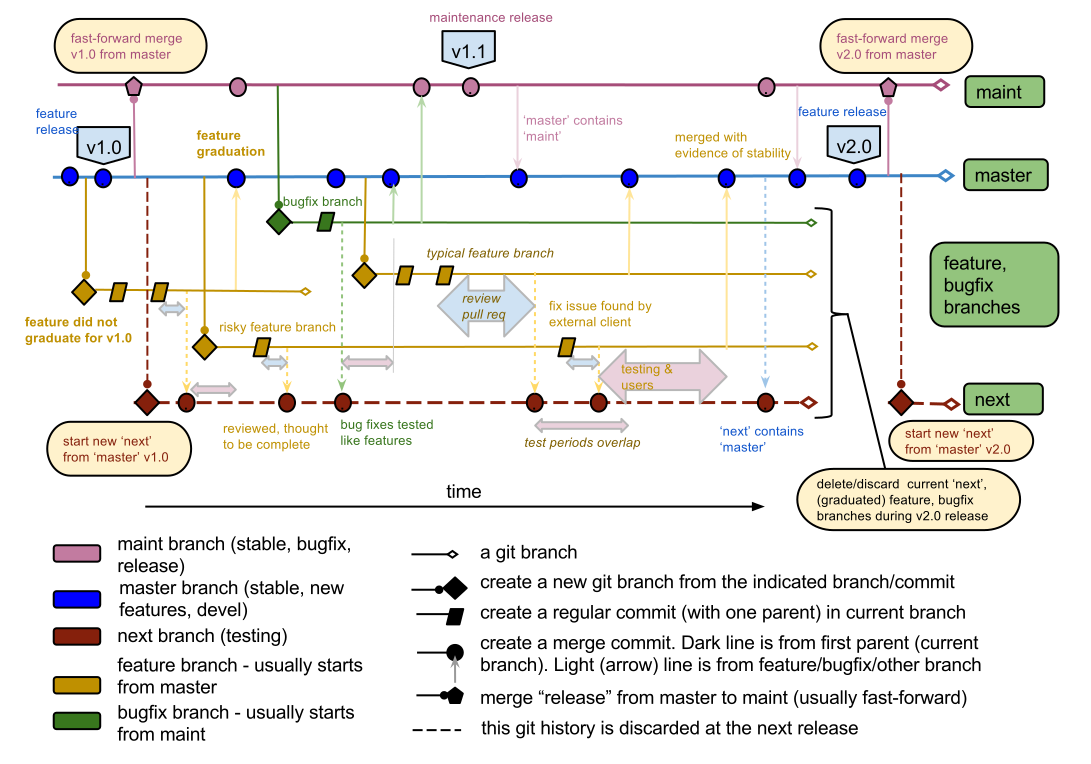
\includegraphics[width=0.85\textwidth]{figures/gitworkflows-satish}
  \end{center}
  \end{block}

  \begin{flushright} \vspace*{-0.5cm}
   \textit{Git is the perl of revision control systems.}
  \end{flushright}
\end{frame}


\begin{frame}{PETSc and Git}
  \begin{center}
    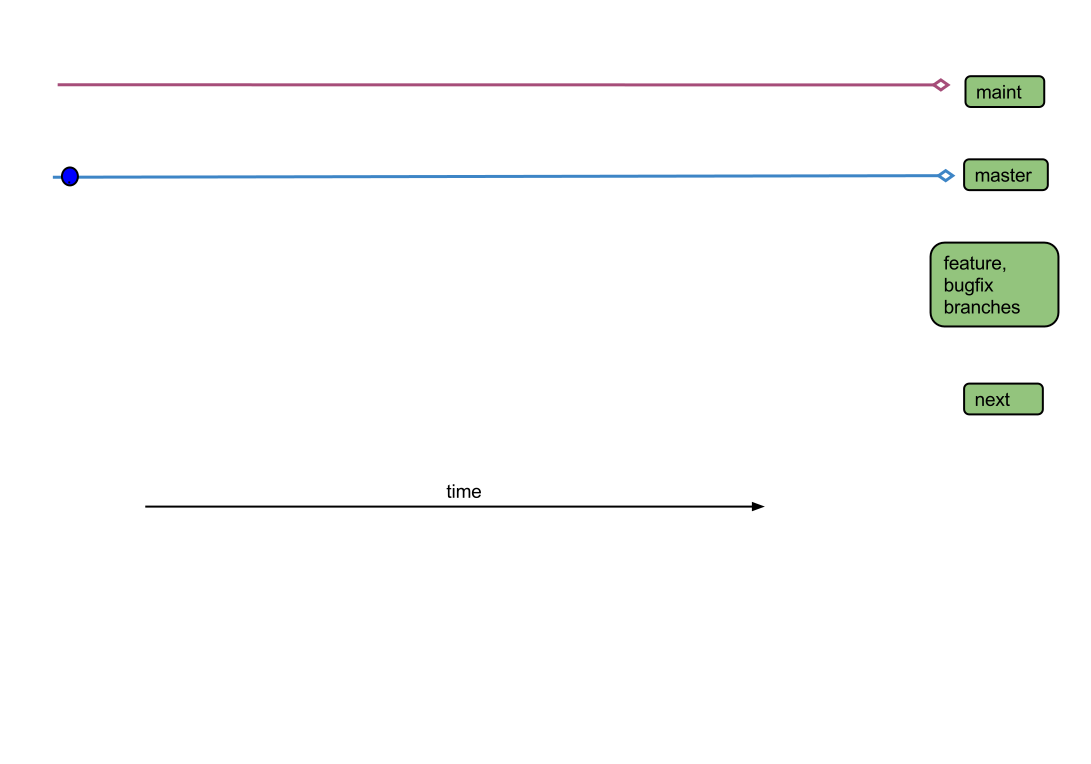
\includegraphics[width=0.99\textwidth]{figures/gitworkflows-45}
  \end{center}
  \begin{flushright} \vspace*{-0.5cm}
   \textit{Oh, yes we all do need that push!}
  \end{flushright}
\end{frame}

\begin{frame}{PETSc and Git}
  \begin{center}
    \includegraphics[width=0.99\textwidth]{figures/gitworkflows-50}
  \end{center}
  \begin{flushright} \vspace*{-0.5cm}
   \textit{It's like we only offer the black belt for people who currently have no belts.}
  \end{flushright}
\end{frame}

\begin{frame}{PETSc and Git}
  \begin{center}
    \includegraphics[width=0.99\textwidth]{figures/gitworkflows-55}
  \end{center}
  \begin{flushright} \vspace*{-0.5cm}
   \textit{If it ain't in email or slashdot then I ain't read it :-)}
  \end{flushright}
\end{frame}

\begin{frame}{PETSc and Git}
  \begin{center}
    \includegraphics[width=0.99\textwidth]{figures/gitworkflows-58}
  \end{center}
  \begin{flushright} \vspace*{-0.5cm}
   \textit{I have now permanently blackholed all email dealing with cygwin.}
  \end{flushright}
\end{frame}

\begin{frame}{PETSc and Git}
  \begin{center}
    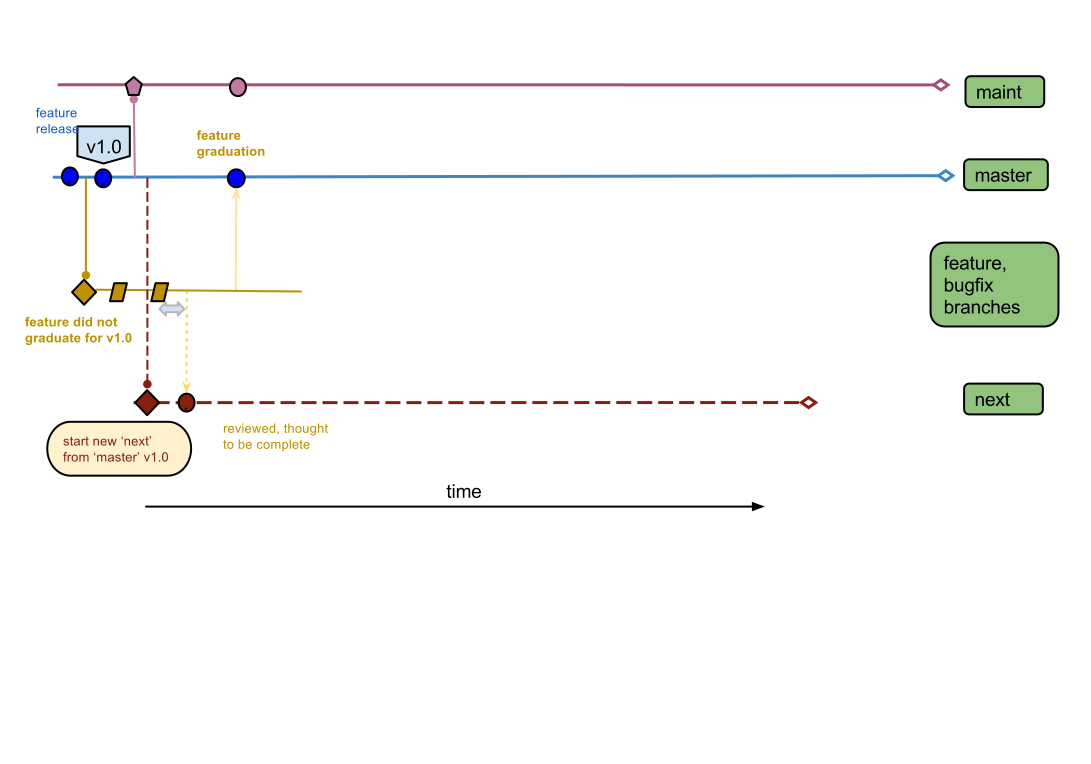
\includegraphics[width=0.99\textwidth]{figures/gitworkflows-60}
  \end{center}
  \begin{flushright} \vspace*{-0.5cm}
   \textit{Peter, Matt gave some bad advice.}
  \end{flushright}
\end{frame}

\begin{frame}{PETSc and Git}
  \begin{center}
    \includegraphics[width=0.99\textwidth]{figures/gitworkflows-65}
  \end{center}
  \begin{flushright} \vspace*{-0.5cm}
   \textit{Satish, please put this in next with the other six million branchs.}
  \end{flushright}
\end{frame}

\begin{frame}{PETSc and Git}
  \begin{center}
    \includegraphics[width=0.99\textwidth]{figures/gitworkflows-70}
  \end{center}
  \begin{flushright} \vspace*{-0.5cm}
   \textit{Don't tell anyone that I put a printf in here}
  \end{flushright}
\end{frame}

\begin{frame}{PETSc and Git}
  \begin{center}
    \includegraphics[width=0.99\textwidth]{figures/gitworkflows-75}
  \end{center}
  \begin{flushright} \vspace*{-0.5cm}
   \textit{I won't call the ICNTL() monstrosity in MUMPS an interface :-)}
  \end{flushright}
\end{frame}

\begin{frame}{PETSc and Git}
  \begin{center}
    \includegraphics[width=0.99\textwidth]{figures/gitworkflows-80}
  \end{center}
  \begin{flushright} \vspace*{-0.5cm}
   \textit{That is all I know about valgrind and it has saved my bacon many times.}
  \end{flushright}
\end{frame}

\begin{frame}{PETSc and Git}
  \begin{center}
    \includegraphics[width=0.99\textwidth]{figures/gitworkflows-85}
  \end{center}
  \begin{flushright} \vspace*{-0.5cm}
   \textit{Stop right here. 99.9\% of the time what you describe should not happen}
  \end{flushright}
\end{frame}

\begin{frame}{PETSc and Git}
  \begin{center}
    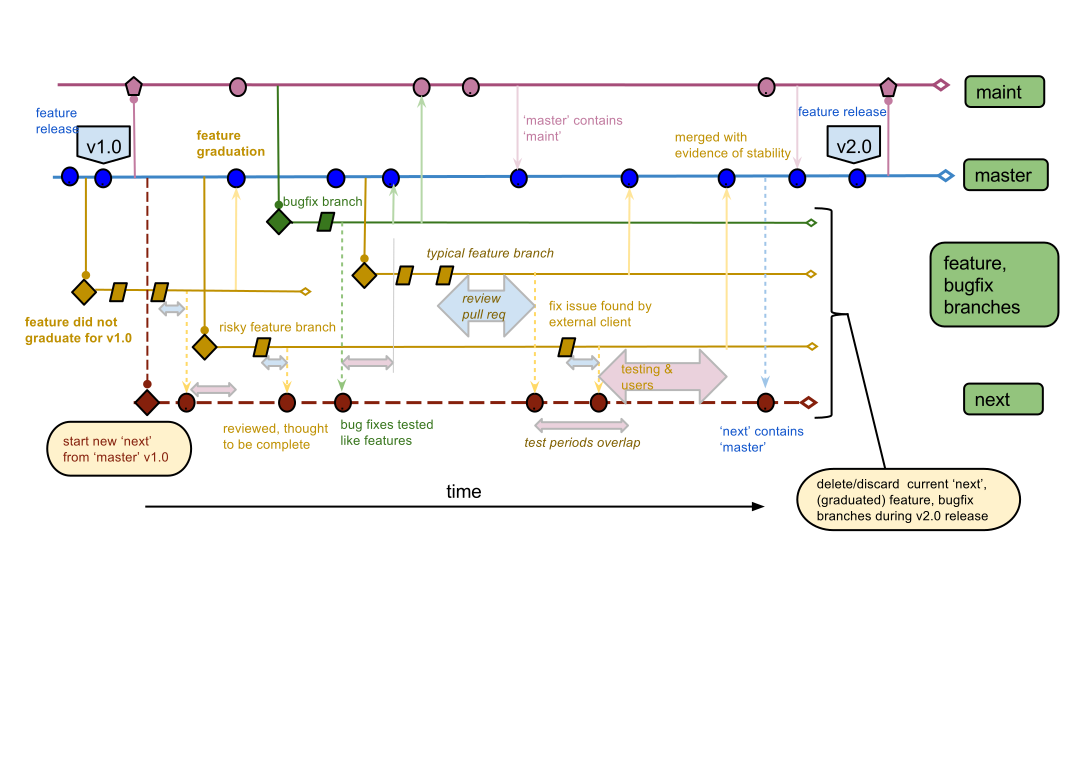
\includegraphics[width=0.99\textwidth]{figures/gitworkflows-90}
  \end{center}
  \begin{flushright} \vspace*{-0.8cm}
   \textit{Git is TeX, what we need is someone to come along\\ and produce LaGit and thus make it usable.}
  \end{flushright}
\end{frame}

\begin{frame}{PETSc and Git}
  \begin{center}
    \includegraphics[width=0.99\textwidth]{figures/gitworkflows-95}
  \end{center}
  \begin{flushright} \vspace*{-1.2cm}
   \textit{Git commands are like irregular verbs in a foreign language: \\
           there’s no all-encompassing logic to them, you just have to memorize \\
           which words you need for each thing you want to express}
  \end{flushright}
\end{frame}

